\documentclass[11pt,letterpaper]{article}
\usepackage[utf8]{inputenc}
\usepackage[T1]{fontenc}
\usepackage{lmodern}
\usepackage{amsmath,amssymb,amsfonts}
\usepackage[margin=2.5cm]{geometry}
\usepackage{fancyhdr}
\usepackage{enumitem}
\usepackage[most]{tcolorbox}
\usepackage{xcolor}
\usepackage{tikz}
\usetikzlibrary{arrows.meta,angles,quotes,calc,positioning}
\usepackage{placeins}
\usepackage{needspace}

% ============ PALETTE: BLACK, ORANGE, AND CREAM ============
\definecolor{blackmain}{HTML}{1A1A1A}
\definecolor{orangeacc}{HTML}{E65C00}
\definecolor{creambg}{HTML}{FBF8F1}
\definecolor{orangebg}{HTML}{FFF4EB}
\definecolor{graymuted}{HTML}{7A746E}
\definecolor{pureblack}{HTML}{0D0D0D}

% ============ HEADERS AND FOOTERS ============
\setlength{\headheight}{24pt}
\pagestyle{fancy}
\fancyhf{}
\fancyhead[L]{\textcolor{blackmain}{\textbf{\small Mathematical Methods I}}}
\fancyhead[R]{\textcolor{orangeacc}{\textbf{\small The Tangent Space}}}
\fancyfoot[C]{\textcolor{graymuted}{\thepage}}
\renewcommand{\headrulewidth}{0.8pt}
\renewcommand{\headrule}{\hbox to\headwidth{\color{orangeacc}\leaders\hrule height \headrulewidth\hfill}}

\setlist[itemize]{label={\small\textcolor{orangeacc}{$\blacksquare$}},leftmargin=1.6em}
\setlist[enumerate]{label={\textcolor{orangeacc}{\arabic*.}},leftmargin=1.8em}

% ============ TITLES ============
\newcommand{\manualsection}[1]{%
  \Needspace{12\baselineskip}%
  \vspace{0.35cm}
  {\Large\bfseries\color{blackmain} #1}\\[2pt]
  {\color{orangeacc}\rule{\linewidth}{1.4pt}}\\[0.25cm]
}

\newcommand{\manualsubsection}[1]{%
  \vspace{0.2cm}\noindent{\bfseries\color{orangeacc} #1}\\[0.12cm]
}

% ============ CONTENT BOXES ============
\newtcolorbox{infobox}[2][orangeacc]{
  enhanced,
  colback=creambg,colframe=#1!90!black,
  boxrule=1pt,arc=2mm,
  left=9pt,right=9pt,top=8pt,bottom=8pt,
  before upper={\textbf{\color{#1!95!black}\large #2}\\[3pt]
    {\color{#1!50}\rule{\linewidth}{0.6pt}}\\[6pt]}
}

\newtcolorbox{theorembox}[1]{
  enhanced,
  colback=creambg!70!white,colframe=pureblack,
  boxrule=1.1pt,arc=2mm,
  left=9pt,right=9pt,top=8pt,bottom=8pt,
  before upper={\textbf{\color{pureblack}\large #1}\\[3pt]
    {\color{orangeacc}\rule{\linewidth}{0.8pt}}\\[6pt]}
}

\newcommand{\term}[1]{\textbf{\color{orangeacc}#1}}
\newcommand{\termb}[1]{\textbf{\color{blackmain}#1}}
\renewcommand{\familydefault}{\rmdefault}
\tikzset{every node/.append style={font=\rmfamily}}

\begin{document}
\color{blackmain}

% ============ TITLE PAGE ============
\begin{center}
  {\LARGE\textbf{\color{blackmain}Mathematical Methods I}}\\[0.2cm]
  {\Large\textcolor{orangeacc}{\textbf{The Tangent Space}}}\\[0.4cm]
  {\large\textcolor{graymuted}{Gabriel Velazquez}}\\[0.6cm]
\end{center}

\manualsection{1. Natural Coordinate Functions}

In Euclidean space $E^n$, the \term{natural coordinate functions}
$x_1,x_2,\ldots,x_n$ assign to each point the value of one of its Cartesian
coordinates. In $E^3$, they are usually denoted by $x$, $y$, and $z$.

\begin{infobox}[orangeacc]{Definition 1.1 (Natural coordinate function)}
Let $p=(p_1,p_2,\ldots,p_n)\in E^n$. The $i$th natural coordinate function is
the function
\begin{equation}
  x_i:E^n\longrightarrow\mathbb{R},
  \qquad x_i(p)=p_i.
\end{equation}
Therefore, every point can be written using the identity
\begin{equation}
  p=\bigl(x_1(p),x_2(p),\ldots,x_n(p)\bigr).
\end{equation}
\end{infobox}

\manualsection{2. Balls, Spheres, and Open Sets}

Differentiability is studied locally. Balls and open sets are used to make precise
what it means to be ``near a point.''

\begin{infobox}[blackmain]{Definition 2.1 (Sphere and balls)}
Given $a\in E^n$ and $r>0$, the equation
\begin{equation}
  \|x-a\|=r
\end{equation}
defines the \term{sphere} of radius $r$ centered at $a$. The corresponding
\term{open ball} and \term{closed ball} are, respectively,
\begin{align}
  B_r(a)&=\{x\in E^n:\|x-a\|<r\},\\
  \overline B_r(a)&=\{x\in E^n:\|x-a\|\le r\}.
\end{align}
The sphere is the common boundary of both balls.
\end{infobox}

\begin{figure}[htbp]
\centering
\begin{tikzpicture}[scale=1.15,>=Stealth]
  \fill[orangebg] (0,0) circle (1.65);
  \draw[orangeacc,very thick] (0,0) circle (1.65);
  \fill[blackmain] (0,0) circle (1.5pt) node[below left] {$a$};
  \draw[->,blackmain,thick] (0,0)--(35:1.65)
    node[midway,above left] {$r$};
  \node[orangeacc] at (0,-2.05) {$B_r(a)$ and its boundary $\|x-a\|=r$};
\end{tikzpicture}
\caption{An open ball contains the points whose distance from the center is less than $r$.}
\label{fig:open-ball}
\end{figure}
\FloatBarrier

\begin{infobox}[orangeacc]{Definition 2.2 (Open set)}
A set $X\subseteq E^n$ is \term{open} if, for every $x\in X$, there exists a
radius $r>0$ such that
\begin{equation}
  B_r(x)\subseteq X.
\end{equation}
A point $x$ belongs to the \termb{boundary} of $X$ if every open ball centered at
$x$, no matter how small, contains at least one point of $X$ and at least one point
that does not belong to $X$. The set $X$ is \term{closed} if it contains all its
boundary points. A \term{neighborhood} of $x$ is an open set containing $x$.
\end{infobox}

\manualsection{3. Differentiable Functions and Maps}

\begin{infobox}[blackmain]{Definition 3.1 (Differentiable function)}
Let $X\subseteq E^n$ be an open set. A real-valued function
$f:X\to\mathbb R$ is called \term{differentiable}, or of class $C^\infty$, if it
has continuous partial derivatives of all orders.
\end{infobox}

In differential geometry, it is common to adopt the convention of working with
$C^\infty$ functions so that derivatives of any order can be computed without
restriction. This is the notion of differentiability used in these notes.

\begin{infobox}[orangeacc]{Definition 3.2 (Differentiable map)}
A map $F:X\subseteq E^n\to E^m$ can be written in terms of its coordinate
functions as
\begin{equation}
  F(p)=\bigl(f_1(p),f_2(p),\ldots,f_m(p)\bigr).
\end{equation}
The map $F$ is \term{differentiable} if each function
$f_j:X\to\mathbb R$ is of class $C^\infty$.
\end{infobox}

\manualsection{4. Tangent Vectors}

A free vector describes only direction and magnitude. For differential calculus,
it is also necessary to record the point in space at which it acts.

\begin{infobox}[orangeacc]{Definition 4.1 (Tangent vector)}
A \term{tangent vector} to $E^n$ is a pair consisting of a point of application
$p\in E^n$ and a vector part $v\in E^n$. It is denoted by
\begin{equation}
  v_p=(p,v).
\end{equation}
Geometrically, it is represented by an arrow with its tail at $p$ and with the
direction and magnitude determined by $v$; its tip is located at $p+v$.
\end{infobox}

\begin{figure}[htbp]
\centering
\begin{tikzpicture}[scale=1.05,>=Stealth]
  \draw[->,graymuted] (-0.4,0)--(5.1,0) node[right] {$x$};
  \draw[->,graymuted] (0,-0.4)--(0,3.5) node[above] {$y$};
  \coordinate (P) at (1.2,0.8);
  \coordinate (Q) at (4.1,2.7);
  \fill[blackmain] (P) circle (1.7pt) node[below] {$p$};
  \draw[->,orangeacc,very thick] (P)--(Q)
    node[midway,above left] {$v_p$};
  \fill[blackmain] (Q) circle (1.7pt) node[right] {$p+v$};
  \draw[dashed,graymuted] (P|-0,0)--(P);
  \draw[dashed,graymuted] (Q|-0,0)--(Q);
\end{tikzpicture}
\caption{The tangent vector $v_p$ is anchored at the point $p$.}
\label{fig:tangent-vector}
\end{figure}
\FloatBarrier

\begin{theorembox}{Dependence on the point of application}
Two tangent vectors with the same vector part but anchored at different points
are distinct objects:
\begin{equation}
  p\ne q \quad\Longrightarrow\quad v_p\ne v_q.
\end{equation}
Therefore, a tangent vector cannot be freely translated without changing it. This
dependence on the point is essential when studying surfaces and manifolds.
\end{theorembox}

\manualsection{5. The Tangent Space}

\begin{infobox}[blackmain]{Definition 5.1 (Tangent space)}
For a fixed $p\in E^n$, the \term{tangent space} at $p$ is the set of all tangent
vectors anchored at that point:
\begin{equation}
  T_p(E^n)=\{v_p:v\in E^n\}.
\end{equation}
\end{infobox}

Because all its elements have the same point of application, the operations
\begin{equation}
  v_p+w_p=(v+w)_p,
  \qquad
  c\,v_p=(cv)_p,
\end{equation}
can be defined, where $v,w\in E^n$ and $c\in\mathbb R$. With these operations,
$T_p(E^n)$ is a vector space.

\begin{figure}[htbp]
\centering
\begin{tikzpicture}[scale=1.05,>=Stealth]
  \coordinate (P) at (0,0);
  \coordinate (V) at (3.2,0.5);
  \coordinate (W) at (1.4,2.4);
  \coordinate (S) at ($(V)+(W)$);
  \draw[->,orangeacc,very thick] (P)--(V) node[midway,below] {$v_p$};
  \draw[->,blackmain,very thick] (P)--(W)
    node[pos=0.58,left=4pt] {$w_p$};
  \draw[->,graymuted,very thick] (P)--(S)
    node[pos=0.6,above right=45pt] {$(v+w)_p$};
  \draw[dashed,graymuted] (V)--(S) (W)--(S);
  \fill[blackmain] (P) circle (1.6pt) node[below left] {$p$};
\end{tikzpicture}
\caption{Addition of vectors within the same tangent space $T_p(E^n)$.}
\label{fig:tangent-addition}
\end{figure}
\FloatBarrier

\begin{theorembox}{Proposition 5.2 (Canonical isomorphism)}
For each fixed point $p$, the map
\begin{equation}
  \Phi_p:E^n\longrightarrow T_p(E^n),
  \qquad \Phi_p(v)=v_p,
\end{equation}
is linear, injective, and surjective. Consequently,
\begin{equation}
  T_p(E^n)\cong E^n,
  \qquad \dim T_p(E^n)=n.
\end{equation}
The isomorphism allows their algebraic structures to be identified, but it does
not eliminate the point of application: $v_p$ still belongs specifically to
$T_p(E^n)$.
\end{theorembox}

\manualsection{6. Vector Fields}

\begin{infobox}[orangeacc]{Definition 6.1 (Vector field)}
A \term{vector field} $V$ on an open set $X\subseteq E^n$ is an assignment that
associates with each point $p\in X$ a tangent vector at that same point:
\begin{equation}
  V:p\longmapsto V(p)\in T_p(E^n).
\end{equation}
Thus, the point of application of $V(p)$ changes along with $p$.
\end{infobox}

\manualsection{7. The Natural Frame}

In $E^3$, consider three constant vector fields pointing in the positive
directions of the Cartesian axes.

\begin{infobox}[blackmain]{Definition 7.1 (Natural vector fields)}
For each $p\in E^3$, define
\begin{equation}
  U_1(p)=(1,0,0)_p,\qquad
  U_2(p)=(0,1,0)_p,\qquad
  U_3(p)=(0,0,1)_p.
\end{equation}
The set $(U_1,U_2,U_3)$ is called the \term{natural frame} or
\term{natural reference frame} of $E^3$.
\end{infobox}

\begin{figure}[htbp]
\centering
\begin{tikzpicture}[scale=1.05,>=Stealth]
  \coordinate (P) at (0,0);
  \draw[->,graymuted] (-2.2,-1.2)--(2.5,1.3) node[right] {$x_1$};
  \draw[->,graymuted] (-2.1,0.8)--(2.6,-1.0) node[right] {$x_2$};
  \draw[->,graymuted] (0,-1.4)--(0,3.1) node[above] {$x_3$};
  \fill[blackmain] (P) circle (1.7pt) node[below left] {$p$};
  \draw[->,blackmain,very thick] (P)--(-1.3,-0.7) node[left] {$U_1(p)$};
  \draw[->,blackmain,very thick] (P)--(1.55,-0.6) node[right] {$U_2(p)$};
  \draw[->,blackmain,very thick] (P)--(0,2.0) node[right] {$U_3(p)$};
\end{tikzpicture}
\caption{The natural frame assigns a basis to each tangent space.}
\label{fig:natural-frame}
\end{figure}
\FloatBarrier

At each point $p$, the vectors $U_1(p),U_2(p),U_3(p)$ form an orthonormal basis of
$T_p(E^3)$. In $E^n$, the natural frame similarly consists of $n$ fields
$U_1,\ldots,U_n$.

\begin{theorembox}{Proposition 7.2 (Canonical representation)}
Every vector field $V$ on $E^n$ can be expressed uniquely as
\begin{equation}
  V=\sum_{i=1}^{n}v_iU_i,
\end{equation}
where $v_1,\ldots,v_n:E^n\to\mathbb R$ are the \term{Euclidean coordinate
functions} of $V$. Evaluating at a point gives
\begin{equation}
  V(p)=\sum_{i=1}^{n}v_i(p)U_i(p).
\end{equation}
\end{theorembox}

For fields $V=\sum_i v_iU_i$ and $W=\sum_i w_iU_i$, and a real-valued function
$f$, the operations are computed componentwise:
\begin{align}
  V+W&=\sum_{i=1}^{n}(v_i+w_i)U_i,\\
  fV&=\sum_{i=1}^{n}(fv_i)U_i.
\end{align}

\manualsection{8. Differentiable Vector Fields}

\begin{infobox}[orangeacc]{Definition 8.1 (Differentiable field)}
Let
\begin{equation}
  V=\sum_{i=1}^{n}v_iU_i
\end{equation}
be a vector field on an open set $X\subseteq E^n$. The field $V$ is
\term{differentiable} if and only if each component function
$v_i:X\to\mathbb R$ is of class $C^\infty$.
\end{infobox}

\end{document}
